% CARVE-VLA WAICA/LNCS-style draft.
% The submitted Agentic-VLA v1 paper is preserved under paper/archive.
\documentclass[runningheads]{waica}

\usepackage[T1]{fontenc}
\usepackage{graphicx}
\usepackage{amsmath,amssymb}
\usepackage{booktabs}
\usepackage{multirow}
\usepackage{tabularx}
\usepackage{url}
\usepackage{xcolor}
\usepackage{etoolbox}

\patchcmd{\thebibliography}{\small}{\footnotesize}{}{}

\newcommand{\method}{CARVE-VLA}
\newcommand{\pizero}{$\pi_{0.5}$}
% Generated by scripts/build_carve_paper_results.py; do not edit manually.
\newcommand{\CarveRealtimeMissReduction}{89.4\%}
\newcommand{\CarveRealtimeWallReduction}{3.7\%}
\newcommand{\CarveSyncEightSuccess}{7/10}
\newcommand{\CarveAsyncSuccess}{5/10}
\newcommand{\CarveAsyncIntervalSuccess}{5/10}
\newcommand{\CarveSyncTenSuccess}{2/2}
\newcommand{\CarveSyncTenRecovery}{1/1}
\newcommand{\CarveCompiledPninetyfive}{67.40~ms}
\newcommand{\CarveSmvePninetyfive}{56.19~ms}
\newcommand{\CarveSmveSuccess}{8/10}
\newcommand{\CarveSmveRuntimeReduction}{16.6\%}
\newcommand{\CarveDroidSmvePninetyfive}{57.34~ms}
\newcommand{\CarveDroidSmveReduction}{13.4\%}
\newcommand{\CarveWMemory}{6.56~GB}
\newcommand{\CarveRecoveryOnlineSuccess}{1/1}
\newcommand{\CarveRecoveryOnlinePninetyfive}{56.41~ms}
\newcommand{\CarveAgenticSmvePninetyfive}{54.50~ms}
\newcommand{\CarveAgenticSmveReduction}{67.2\%}
\newcommand{\CarveFullAgenticSuccess}{183/400}
\newcommand{\CarveFullFrozenSuccess}{180/400}
\newcommand{\CarveFullConversions}{4}
\newcommand{\CarveFullRegressions}{1}
\newcommand{\CarveFullMcnemar}{0.375}
\newcommand{\CarveFullCallReduction}{8.4\%}
\newcommand{\CarveFullStepReduction}{7.2\%}
\newcommand{\CarveFullVlaPninetyfive}{59.54~ms}
\newcommand{\CarveFullPlannerPninetyfive}{11.23~s}
\newcommand{\CarveFinalSmvePninetyfive}{54.67~ms}
\newcommand{\CarveFinalSmveReduction}{80.6\%}
\newcommand{\CarvePlannerNfMemoryReduction}{63.6\%}
\newcommand{\CarveLowMemoryPair}{11.22~GiB}
\newcommand{\CarveLowMemoryVlaLatency}{66.69~ms}


\begin{document}

\title{CARVE-VLA: A Compute-Aware Agentic Runtime for Reliable and Efficient VLA Execution}
\titlerunning{CARVE-VLA}

% Double-blind placeholder. Replace after the review policy is finalized.
\author{Anonymous Authors}
\authorrunning{Anonymous Authors}
\institute{Anonymous Institution}

\maketitle

\begin{abstract}
Vision-language-action (VLA) policies provide strong local manipulation skills,
but long-horizon deployment requires both execution supervision and a feasible
control-loop latency. Agentic wrappers can monitor progress and recover from
failure, yet their additional inference and verification can make this timing
problem worse. We present \method{}, a model-agnostic runtime that co-designs
an Agentic Harness with an Optimize Runtime around a frozen VLA. A high-rate
monitor processes deployable execution signals, while an event-triggered VLM
Planner performs low-rate semantic assessment only at safe boundaries. Typed
gates constrain planner outputs to VLA calls, registered recovery skills, or
safe stop; structured failure memory supplies bounded evidence but never emits
actions. The Optimize Runtime admits hardware-bound profiles through fidelity,
latency, and closed-loop gates before deployment.

We evaluate the frozen policy, fixed recovery, and the full Agentic runtime on
the same 400 initial states spanning the clean, Object-OOD, Swap-OOD, and
Task-OOD suites: 1,200 interactive MuJoCo episodes in total. Full Agentic
execution reaches \CarveFullAgenticSuccess{} versus
\CarveFullFrozenSuccess{}, with \CarveFullConversions{} corrected failures and
\CarveFullRegressions{} regression (exact McNemar $p=\CarveFullMcnemar$).
The success difference is not statistically significant; however, the
Agentic branch reduces VLA calls by \CarveFullCallReduction{} and executes 263
guarded semantic-planning events without privileged simulator state. Separate
efficiency experiments on an RTX 4090 show that two-step compiled BF16 with
static masked-view elision (SMVE) reduces PI0.5 P95 from 282.43 ms to
\CarveFinalSmvePninetyfive{} (\CarveFinalSmveReduction{}), eliminates all
80-ms misses on 45 paired observations, and preserves every checked action.
For the Qwen3.5-4B Planner, NF4 reduces model memory by
\CarvePlannerNfMemoryReduction{} with exact semantic-decision agreement, but
increases P95 from 1.90 to 2.91 s and is retained only as a memory tier. A real
co-resident NF4-Planner/SMVE-VLA dry run occupies \CarveLowMemoryPair{} and
meets the VLA deadline at \CarveLowMemoryVlaLatency{}; actions are deliberately
withheld, so this result establishes integration feasibility rather than task
success. These results support a bounded conclusion: execution supervision and
efficient inference can be composed around a frozen VLA, but profile admission
must jointly test semantics, latency, memory, and closed-loop behavior.

\keywords{Vision-language-action models \and Agentic policy \and Robot manipulation \and Long-horizon control \and Efficient inference}
\end{abstract}

\section{Introduction}
\label{sec:intro}

Vision-language-action (VLA) policies couple perception, language grounding, and low-level control within a single action model.
RT-1 and RT-2 demonstrated large-scale visuomotor policies and web-knowledge transfer to robot control~\cite{brohan2022rt1,brohan2023rt2}.
Open X-Embodiment, Octo, OpenVLA, \pizero{}, and \pizero{}-style policies have further made generalist robot policies increasingly accessible~\cite{oneill2023openx,octo2024octo,kim2024openvla,black2024pi0,physicalintelligence2025pi05}.
Once such policies become strong on short-horizon skills, the next question is no longer whether a robot can execute one local behavior, but whether it can organize many local behaviors into a reliable long-horizon process.

Long-horizon manipulation exposes failures that are easy to miss in atomic tasks.
Benchmarks such as CALVIN and LIBERO require skill chaining, temporal coherence, and recovery from off-nominal states~\cite{mees2021calvin,liu2023libero}.
Recent long-horizon VLA analyses make the same point: stronger action models improve local competence, yet subtask handoff, accumulated drift, and recovery remain persistent bottlenecks~\cite{fan2025longvla,han2025robocerebra}.
For a strong fine-tuned VLA, many residual failures are therefore better described as missing \emph{process control} rather than missing low-level control.
The policy may know how to reach, grasp, or place, but the execution loop may not know when progress has stalled, when a transition motion is needed, when a task-specific prior should be injected, or when the current attempt should be retried.

This paper frames the issue as an \emph{execution-supervision problem} for frozen VLAs:
\begin{quote}
\emph{How should a strong frozen VLA be embedded in a monitored, recoverable, and realtime-aware long-horizon execution loop?}
\end{quote}
The framing matters because it separates two roles that are often conflated.
The VLA is the local action generator.
The runtime is responsible for progress monitoring, context injection, recovery, call scheduling, and evidence logging.
This separation is especially relevant when the available compute budget cannot support retraining a foundation-scale robot policy, but can support a careful control layer around it.

We instantiate this idea as \method{}, a Compute-Aware Agentic Runtime for VLA
Execution. Its Agentic Harness combines high-frequency risk monitoring with a
low-frequency event-triggered VLM Critic/Planner, typed failure memory, bounded
physical recovery, and safe hold. Its Optimize Runtime admits a hardware-bound
inference profile and executes it with explicit deadline, fallback, and tracing
contracts. The two layers meet only through typed observations, actions,
capabilities, deadlines, and Agentic-event traces.
This boundary lets the same Harness wrap another chunked VLA while preventing
an unsupported optimization from being silently reported as active. All
modules operate around the original policy server; the VLA backbone remains
frozen.

\begin{figure}
    \centering
    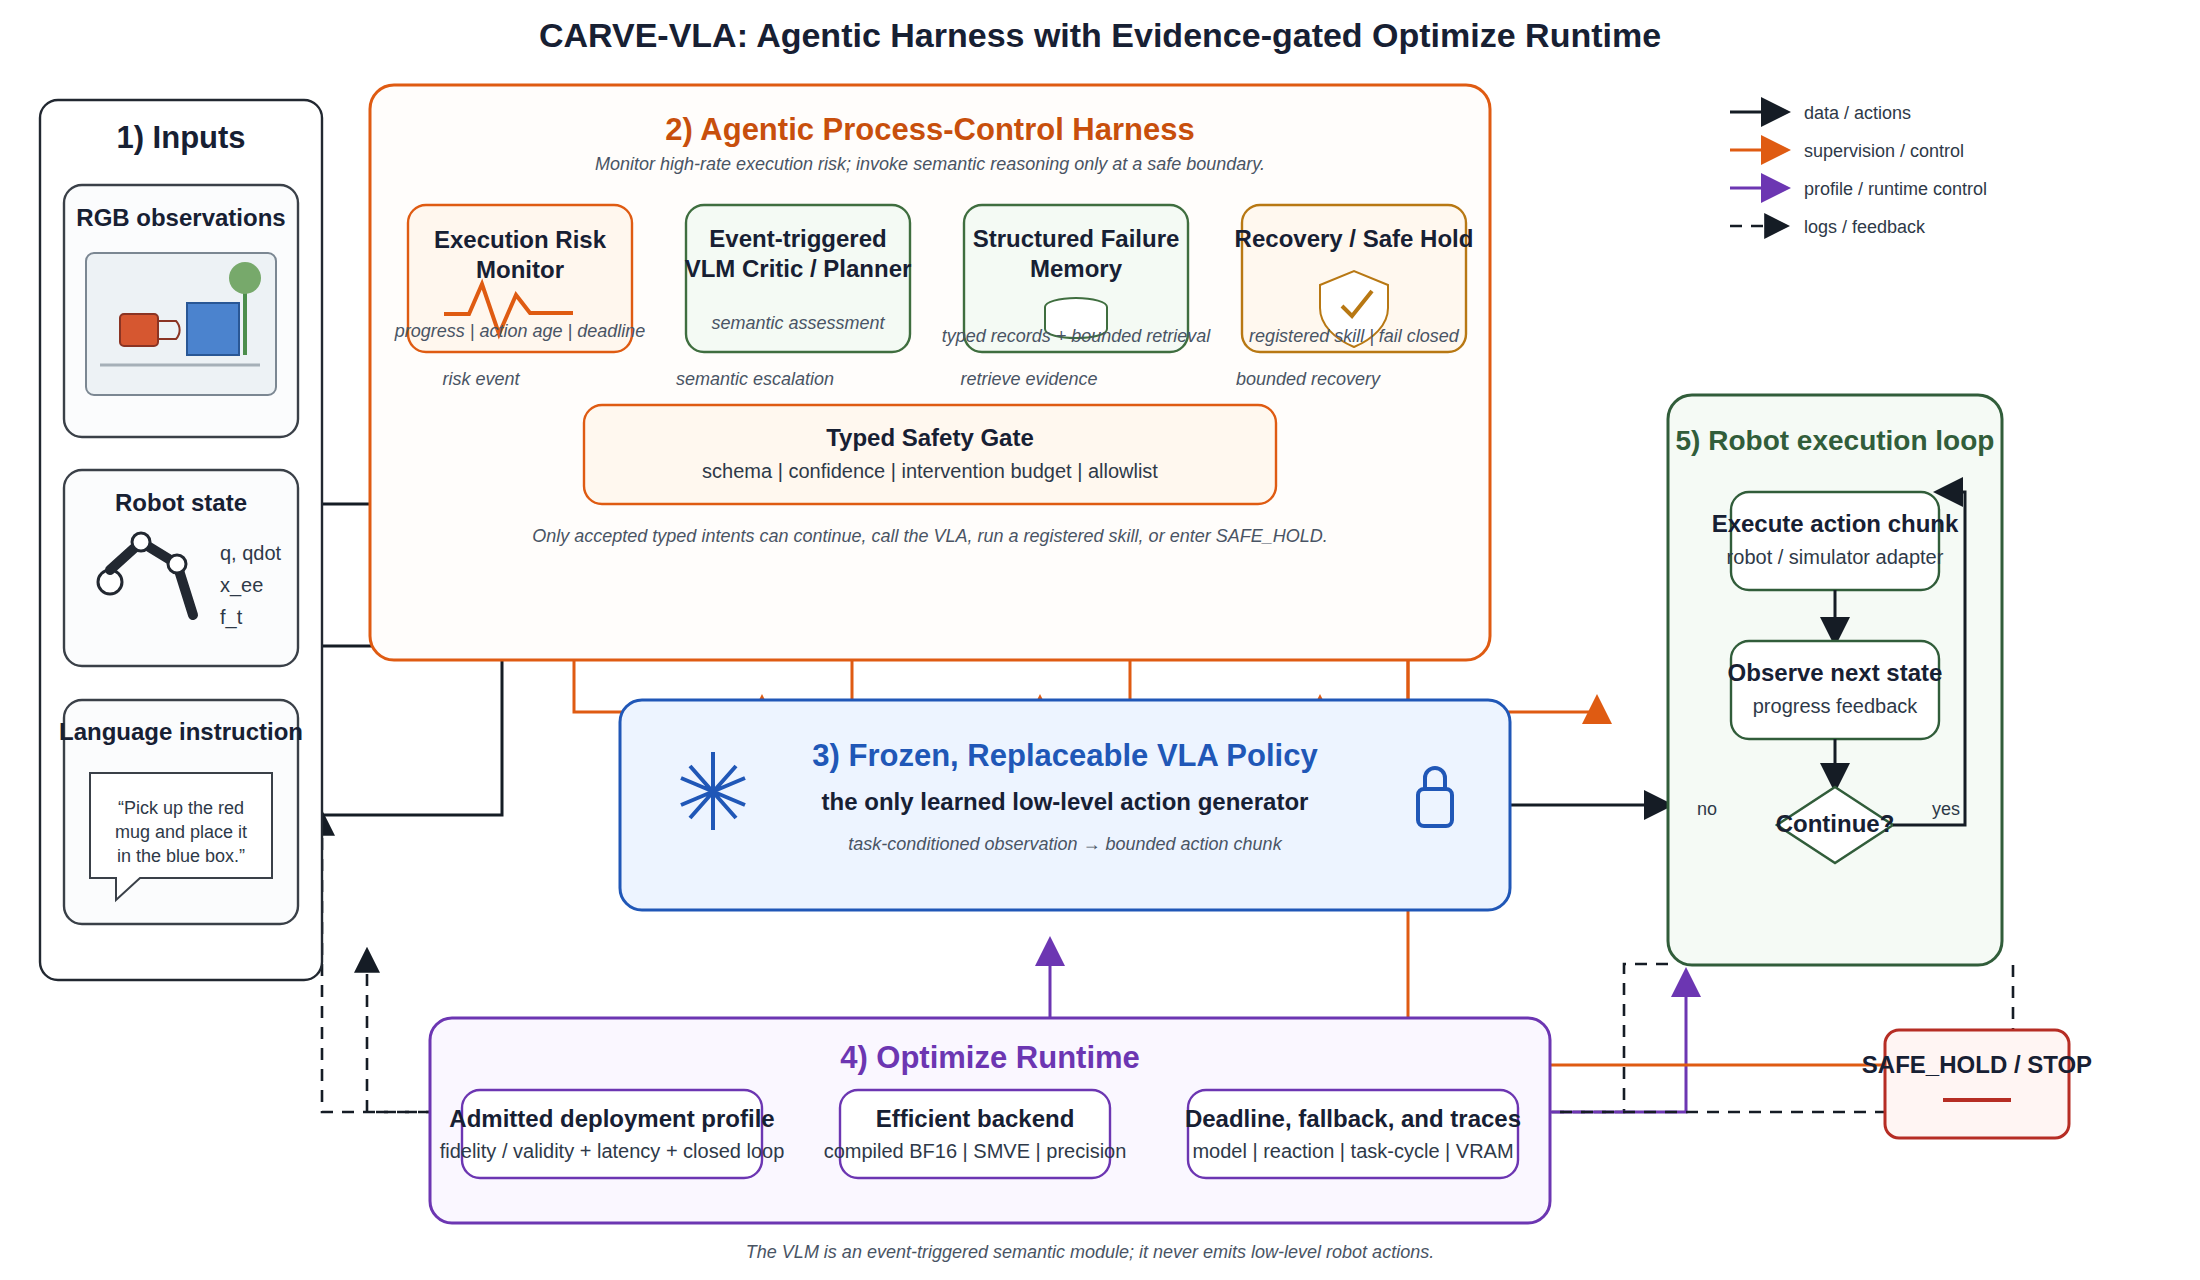
\includegraphics[width=0.96\textwidth]{figures/fig1_framework_fused.png}
    \caption{Overview of \method{}.
    The replaceable frozen VLA remains the only learned low-level action
    generator. The multi-rate Agentic Harness supervises execution and bounded
    recovery, while the independently usable Optimize Runtime admits and traces
    efficient VLA/VLM deployment profiles.}
    \label{fig:overview}
\end{figure}

Our contributions are:
\begin{itemize}
    \item We formulate frozen-VLA deployment as a joint
    execution-supervision and control-latency problem, and expose a reusable
    boundary among action semantics, model capabilities, Agentic events,
    deadlines, fallbacks, and traces.
    \item We instantiate this formulation as a multi-rate Agentic Harness:
    deterministic execution monitoring remains on the high-rate path; a
    guarded VLM Planner, structured failure memory, HAA-RAG knowledge, and
    typed physical skills are invoked only at explicit safe boundaries.
    \item We develop an evidence-gated Optimize Runtime that binds every
    candidate to a checkpoint, adapter, hardware contract, flow-step budget,
    and action horizon. Replay fidelity, warm runtime, and paired closed-loop
    outcomes jointly decide profile admission.
    \item We provide a paired 1,200-episode official LIBERO/LIBERO-PRO study,
    exact-state recovery tests, PI0.5 and Planner precision ablations, and a
    real co-resident Planner--VLA integration gate. Positive, null, and rejected
    results remain separated by explicit evidence boundaries.
\end{itemize}

\section{Related Work}
\label{sec:related}

\paragraph{Foundation VLA policies.}
Modern VLA research has progressed from RT-1 and RT-2 to open and generalist policy stacks such as Octo, OpenVLA, \pizero{}, and \pizero{}~\cite{brohan2022rt1,brohan2023rt2,octo2024octo,kim2024openvla,black2024pi0,physicalintelligence2025pi05}.
Open X-Embodiment and related efforts emphasize shared datasets and cross-robot policy learning~\cite{oneill2023openx}.
These models make frozen or lightly adapted VLA policies strong enough that remaining failures become more diagnostically useful: when local skills are present, long-horizon performance depends increasingly on execution organization.

\paragraph{Long-horizon benchmarks.}
CALVIN and LIBERO evaluate language-conditioned manipulation across temporally extended tasks~\cite{mees2021calvin,liu2023libero}.
Long-VLA and RoboCerebra further emphasize that temporal consistency, state transitions, and off-nominal recovery remain difficult even for strong policies~\cite{fan2025longvla,han2025robocerebra}.
Our main evaluation uses LIBERO because it provides official interactive rollouts, task-level success signals, and a challenging but reproducible long-horizon suite.

\paragraph{Agentic augmentation and memory.}
Agentic robot systems augment policy execution with planners, verifiers, memory, tools, or online adaptation~\cite{yang2025agenticrobot,li2026roboclaw,pang2026scivla,jin2026agenticvla}.
Embodied memory work studies how short-term and long-term memory can support manipulation~\cite{torne2026mem,shi2025memoryvla}.
\method{} is aligned with this direction but takes a conservative stance: modules remain lightweight, execution-time, and attributable to rollout events rather than absorbed into a new monolithic planner.

\paragraph{Failure detection and efficient inference.}
Failure-aware systems use VLMs or specialized monitors to detect execution errors, reason about failures, and trigger recovery~\cite{duan2024aha,grislain2025ifailsense,lin2025failsafe}.
ECoT and Fast ECoT show that explicit embodied reasoning can also improve action generation and efficiency~\cite{zawalski2024ecot,duan2025fastecot}.
Realtime robot control imposes constraints that are not captured by success rate alone.
Recent efficient VLA work studies caching, low-latency decoding, and realtime diffusion-policy execution~\cite{xu2025vlacache,guan2025efficientvlasurvey,niu2026realtimevlaflash,yang2026realtimevlav2}.
Our runtime study is complementary: instead of treating kernel speed, low-step
sampling, or quantization as sufficient in isolation, we require action-level
fidelity and paired closed-loop behavior before a profile can serve the
Agentic execution loop.

\section{Method}
\label{sec:method}

\subsection{Frozen Policy and Chunked Execution}

The baseline policy is a frozen \texttt{pi05\_libero} policy derived from the \pizero{} family and served through the OpenPI stack.
At control step $t$, the policy receives visual observations $o_t$, robot state $s_t$, and language instruction $\ell$, and predicts an action chunk
\begin{equation}
A_t = \pi_\theta(o_t,s_t,\ell) =
(a_t,a_{t+1},\ldots,a_{t+H-1}).
\end{equation}
The executor applies part of the chunk before replanning.
This scheme is effective for many short and medium-horizon tasks, but it can fail when locally plausible chunks do not smoothly connect adjacent subtask states.
\method{} repairs this failure mode without changing $\pi_\theta$: the backbone remains frozen, and external modules intervene only at inference time.

\subsection{Problem Formulation and Authority Separation}

Let $x_t=(o_t,s_t,q_t)$ denote the deployable observation, robot state, and
remaining action queue at control step $t$. The runtime selects an execution
mode $m_t$ from cached execution, VLA inference, one registered physical skill,
semantic planning, or safe stop. We seek a runtime policy $\rho$ that improves
task completion while controlling inference cost and intervention risk,
\begin{equation}
\max_{\rho}\quad
\mathbb{E}\!\left[S(\tau)\right]
-\lambda_L C_{\mathrm{lat}}(\tau)
-\lambda_I C_{\mathrm{int}}(\tau)
-\lambda_U C_{\mathrm{unsafe}}(\tau),
\label{eq:objective}
\end{equation}
subject to an action contract, per-episode planner/recovery budgets, and a
deadline $d$ for every admitted VLA call. Here $S(\tau)$ is evaluator-side task
success and is never available to the online controller. Equation~\ref{eq:objective}
is a systems objective rather than a learned loss: the present implementation
uses auditable rules and offline profile gates to enforce it.

The authority boundary is strict. The VLA is the only learned module allowed
to produce low-level action chunks. A registered physical skill may emit only
actions inside its declared \texttt{ActionSpec}. The VLM may select a local VLA
instruction, a registered skill, continued execution, or safe stop, but cannot
emit actions, joint targets, torques, or trajectories. Memory and retrieval
provide evidence only. This decomposition prevents a fluent planner response
from bypassing robot-specific action semantics.

\begin{table}
\caption{Multi-rate modules, inputs, outputs, and execution authority.}
\label{tab:authority}
\centering
\small
\begin{tabularx}{\textwidth}{p{0.18\textwidth}p{0.17\textwidth}p{0.25\textwidth}X}
\toprule
Component & Typical rate & Output & Authority \\
\midrule
Monitor & every control step & risk score, event, evidence & observes only; never acts \\
VLA runtime & per action chunk & validated $H\!\times\!D$ action chunk & learned low-level actions \\
VLM Planner & event-only & typed intent and semantic subgoal & chooses only allowed executors \\
Recovery skill & bounded event & contract-checked action phases & analytic actions within one skill envelope \\
Memory / HAA-RAG & safe boundary & bounded evidence records & no execution authority \\
\bottomrule
\end{tabularx}
\end{table}

\subsection{Execution-Supervision Loop}

The key algorithmic object is the execution-supervision loop in Fig.~\ref{fig:execution_loop}.
During normal progress, a deterministic high-rate monitor evaluates
proprioceptive response, commanded motion, action age, optional uncertainty,
and deadline slack. The admitted VLA profile generates a bounded action chunk,
the robot executes it, and the next deployable observation closes the loop.
Simulator object poses and task-success predicates are excluded from online
control.

A risk event enters an explicit state machine. The controller first verifies
the evidence, then selects an accurate VLA replan, a registered bounded
recovery skill, or semantic escalation. Semantic escalation occurs only at a
safe boundary: an asynchronous VLM Critic/Planner receives the task, frames,
monitor evidence, bounded memory, remaining budgets, and current skill
allowlist. A typed safety gate accepts only \texttt{continue},
\texttt{vla\_act}, \texttt{run\_skill}, or \texttt{safe\_stop}. Malformed,
uncertain, stale, timed-out, or budget-exhausted decisions fail closed through
\texttt{SAFE\_HOLD} and \texttt{STOP}. The VLM never emits a robot action.

\begin{figure}
    \centering
    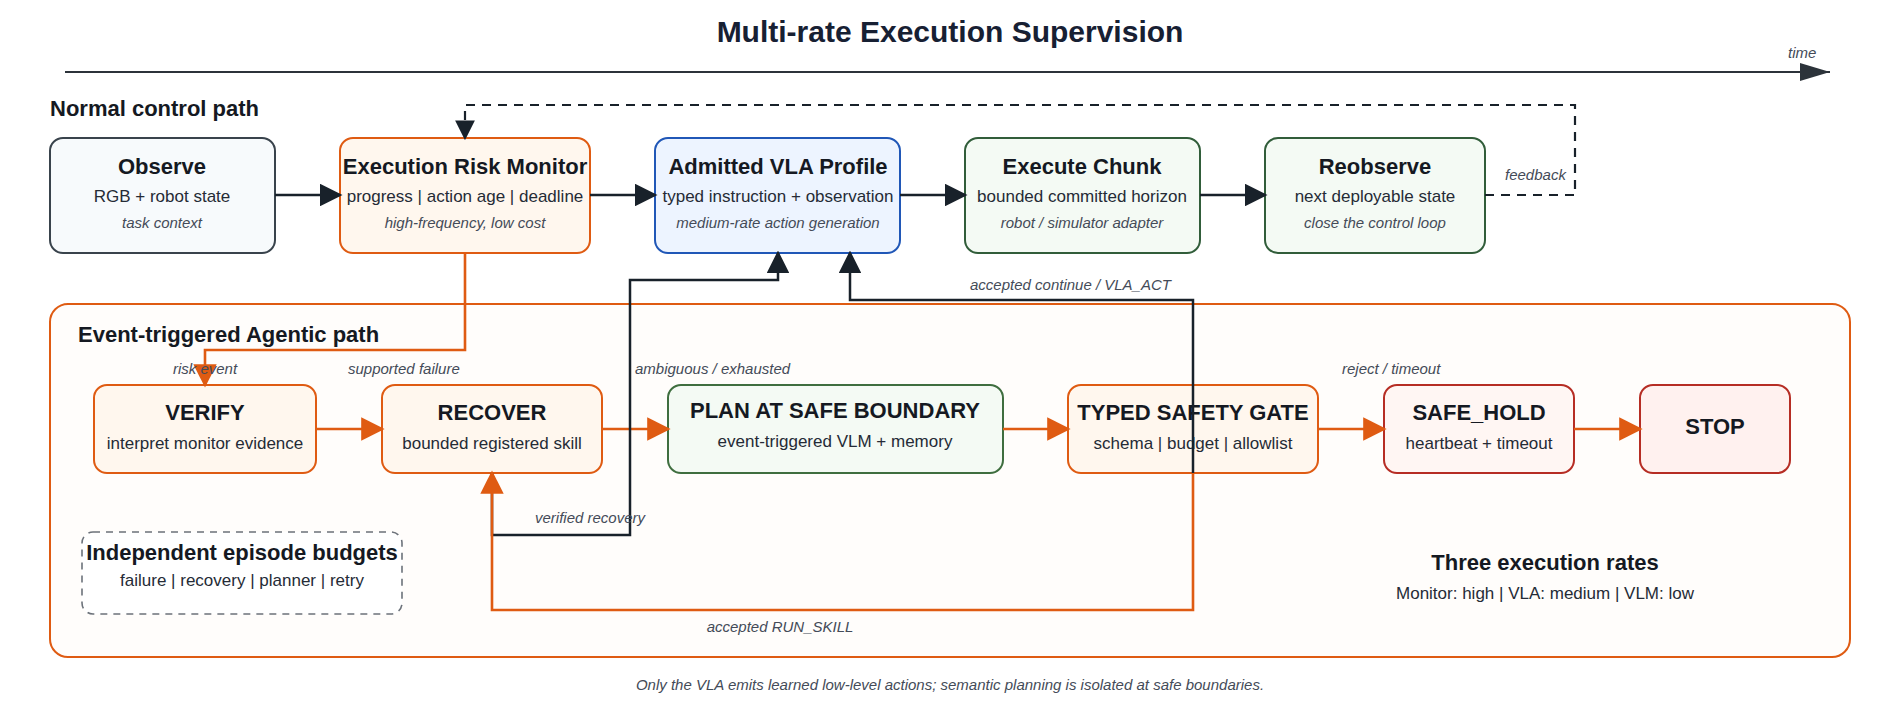
\includegraphics[width=0.94\textwidth]{figures/fig2_execution_supervision_v2.png}
    \caption{Multi-rate execution-supervision loop. High-frequency monitoring
    keeps routine semantic calls off the control path. Confirmed events trigger
    bounded recovery or low-frequency VLM planning at a safe boundary; typed
    acceptance, independent budgets, and safe hold make every transition
    auditable and fail closed.}
    \label{fig:execution_loop}
\end{figure}

\subsection{Deployable Monitor and Multi-Rate State Machine}

The Monitor compares commanded motion with observed response over a sliding
window. Let $u_t$ be the commanded action without its gripper dimension,
$p_t$ proprioception, and $I_t$ the optional RGB frame. The implementation
computes
\begin{align}
c_t &= \lVert u_t\rVert_2, &
r_t^p &= \lVert p_t-p_{t-1}\rVert_2,\\
r_t^v &= \frac{1}{|I|}\lVert I_t-I_{t-1}\rVert_1.
\end{align}
A stall is declared only after monitor warm-up when the windowed command is
large but both proprioceptive and available visual responses remain below
threshold. This is deliberately symptom detection, not semantic diagnosis.
Action staleness, optional model uncertainty, and deadline pressure form the
remaining normalized risks. The aggregate is
\begin{equation}
R_t = 0.45R_t^{\mathrm{stall}}+0.20R_t^{\mathrm{age}}
      +0.20R_t^{\mathrm{unc}}+0.15R_t^{\mathrm{ddl}},
\label{eq:risk}
\end{equation}
with low/medium/high buckets at $0.35$ and $0.65$. Missing uncertainty or
deadline information contributes zero rather than being hallucinated. The
PRO qualification uses a 60-step event warm-up to avoid startup transients;
all response evidence is still logged during that interval.

The episode controller owns independent failure, recovery, planner-call, and
semantic-retry counters. Table~\ref{tab:states} makes the state semantics
explicit. A planner request is single-flight and carries an episode/timestep
ticket. Results that are stale, malformed, timed out, below the intervention
confidence threshold, outside the intent/skill allowlist, or beyond budget are
rejected. In a real robot adapter, \texttt{SAFE\_HOLD} must define a stationary
command, heartbeat, timeout, release, and stop operation; in LIBERO it is
implemented as a paused safe boundary and is named as such in the trace.

\begin{table}
\caption{Canonical Agentic Harness states and exit conditions.}
\label{tab:states}
\centering
\small
\begin{tabularx}{\textwidth}{p{0.22\textwidth}p{0.32\textwidth}X}
\toprule
State & Operation & Allowed exit \\
\midrule
\texttt{EXECUTE\_FAST} & execute a validated VLA chunk or cached suffix & continue, \texttt{VERIFY}, or \texttt{STOP} \\
\texttt{VERIFY} & confirm monitor evidence and available budgets & VLA replan, \texttt{RECOVER}, planner boundary, or stop \\
\texttt{RECOVER} & execute one registered bounded skill and verify response & fresh VLA replan or safe hold \\
\texttt{PLAN/BOUNDARY} & submit/poll one typed VLM request & apply accepted intent or safe hold \\
\texttt{SAFE\_HOLD} & maintain adapter-defined stationary behavior & explicit release, timeout, or stop \\
\texttt{STOP} & terminal fail-closed state & none \\
\bottomrule
\end{tabularx}
\end{table}

\subsection{Failure Taxonomy}

\method{} is organized around a concrete failure taxonomy rather than a generic ``reasoning helps'' claim.
We distinguish four recurring long-horizon failure modes:
\textit{transition failures}, where adjacent subtask phases do not connect smoothly;
\textit{contact or grasp failures}, where object interaction is locally unstable;
\textit{completion failures}, where the object is moved but the terminal condition is not reached; and
\textit{recovery failures}, where a failed segment is detected but the system cannot re-enter a useful state.
Table~\ref{tab:taxonomy} maps these failures to modules and expected evidence.

\begin{table}
\caption{Failure modes are tied to observable rollout evidence rather than post-hoc labels.}
\label{tab:taxonomy}
\centering
\small
\begin{tabularx}{\textwidth}{p{0.22\textwidth}p{0.30\textwidth}p{0.22\textwidth}X}
\toprule
Failure mode & Observable signal & Helpful module & Expected ablation signal \\
\midrule
Transition gap & low recent motion near a subtask boundary; repeated replans without phase change & monitor + bounded recovery & recovery should restore a responsive state before replanning \\
Contact ambiguity & object is reached but grasp/place geometry remains unstable & VLM Planner + memory & typed intervention should outperform blind repeated replanning \\
Incomplete rollout & object is manipulated but terminal condition is not achieved & VLM Planner / VLA retry & accepted subgoal repair should change the subsequent rollout \\
Derailment & rollout state inconsistent with task progress after an intervention & verification + safe hold & failed verification should prevent another unsafe action \\
\bottomrule
\end{tabularx}
\end{table}

This taxonomy defines how the method should be falsified.
If a module is claimed to repair a failure mode, the corresponding rollout signal should change in the logs or in a targeted ablation.
For example, useful recovery must change a measured post-intervention response,
while a useful semantic planner must produce accepted decisions that alter a
paired rollout without increasing unsafe interventions. The earlier LIBERO-10
configuration used deterministic transition, prior, and critic modules; we
retain its completed benchmark as historical Harness evidence but do not
attribute those outcomes to the newly added VLM Planner.

\subsection{Process-Control Modules}

Fig.~\ref{fig:modules} separates four responsibilities that are easy to
conflate. The \emph{Execution Risk Monitor} is deterministic and high rate. It
uses deployable temporal signals and produces a risk score, bucket, event, and
evidence; it is not a semantic scene reasoner. The \emph{VLM Critic/Planner} is
low rate and event triggered. It sees images and task meaning, but a typed gate
prevents it from returning raw robot actions or unregistered tools.

The planner context contains the original task, current subgoal, named RGB
frames, proprioception, measured risk, failure history, bounded memory records,
qualitative scene graph, HAA-RAG cards, remaining budgets, current deployment
profile, deadline slack, allowed intents, and registered-skill names. It returns
one compact JSON decision. Table~\ref{tab:intents} shows how that decision is
grounded. The original task is never replaced: accepted local guidance is
appended as ``current recovery subgoal'' before the next VLA call. This avoids
turning a short repair instruction into a new, incomplete task specification.

\begin{table}
\caption{Guarded VLM intents. The gate validates schema, confidence, budget,
allowlist membership, freshness, and absence of raw actions.}
\label{tab:intents}
\centering
\small
\begin{tabularx}{\textwidth}{p{0.18\textwidth}p{0.30\textwidth}X}
\toprule
Intent & Required field & Harness effect \\
\midrule
\texttt{continue} & rationale, confidence & retain current objective; issue no new action itself \\
\texttt{vla\_act} & validated local instruction & append grounded subgoal and call the frozen VLA \\
\texttt{run\_skill} & registered \texttt{skill\_id} & invoke only the named bounded skill \\
\texttt{safe\_stop} & rationale & enter hold/terminal stop without another learned action \\
\bottomrule
\end{tabularx}
\end{table}

The \emph{Structured Failure Memory} stores typed
\texttt{FailureEpisodeRecord}s containing context/profile identity, failure
evidence, action age, intervention budget, verification, outcome, confidence,
timestamp, and expiry. Retrieval is bounded by context, failure type,
deployment profile, and validity period. It may change planner context or
suppress a failed intervention, but cannot issue an action.

Semantic knowledge is similarly constrained. A deployable scene graph stores
entities and qualitative relations such as inside, near, supported-by, and
grasped-by; it excludes metric poses,
reward, success, simulator state, trajectories, and joint targets. HAA-RAG
stores affordance cards with object categories, grasp regions, material,
fragility, applicable failures, constraints, and prior outcome. Training-free
retrieval ranks a card by task/scene category overlap, failure match, and card
confidence,
\begin{equation}
\mathrm{score}(e)=2N_{\mathrm{cat}}(e)+1.5\,\mathbb{1}_{\mathrm{fail}}(e)
                   +0.25\,c(e).
\label{eq:haa}
\end{equation}
When any task- or scene-matched card exists, failure-only cards for unrelated
objects are suppressed. This prevents a generic past failure from dominating
current object semantics.

The initial preserve-grasp skill,
\path{cartesian_retract_lift_reobserve}, declares an action specification,
preconditions, supported failures, timeout, maximum actions, verification rule,
and fail-closed behavior. It executes stabilize, retract, lift, and reobserve
phases. Only a verified deployable state response permits a fresh VLA replan;
failure or timeout enters safe hold. This is one registered skill rather than a
claim of a general skill library.

The default registry contains preserve-grasp and release-and-retreat variants.
Selection is constrained by the
failure type and planner allowlist. The preserve-grasp plan applies 2 stabilize,
4 retract, 4 lift, and 2 settle/reobserve actions. Every vector is finite,
dimension checked, and projected to the declared normalized range. Verification
uses measured end-effector response rather than task success. Thus a skill can
successfully restore controllability even if the long-horizon task later fails;
the two outcomes are intentionally logged separately.

\begin{figure}
    \centering
    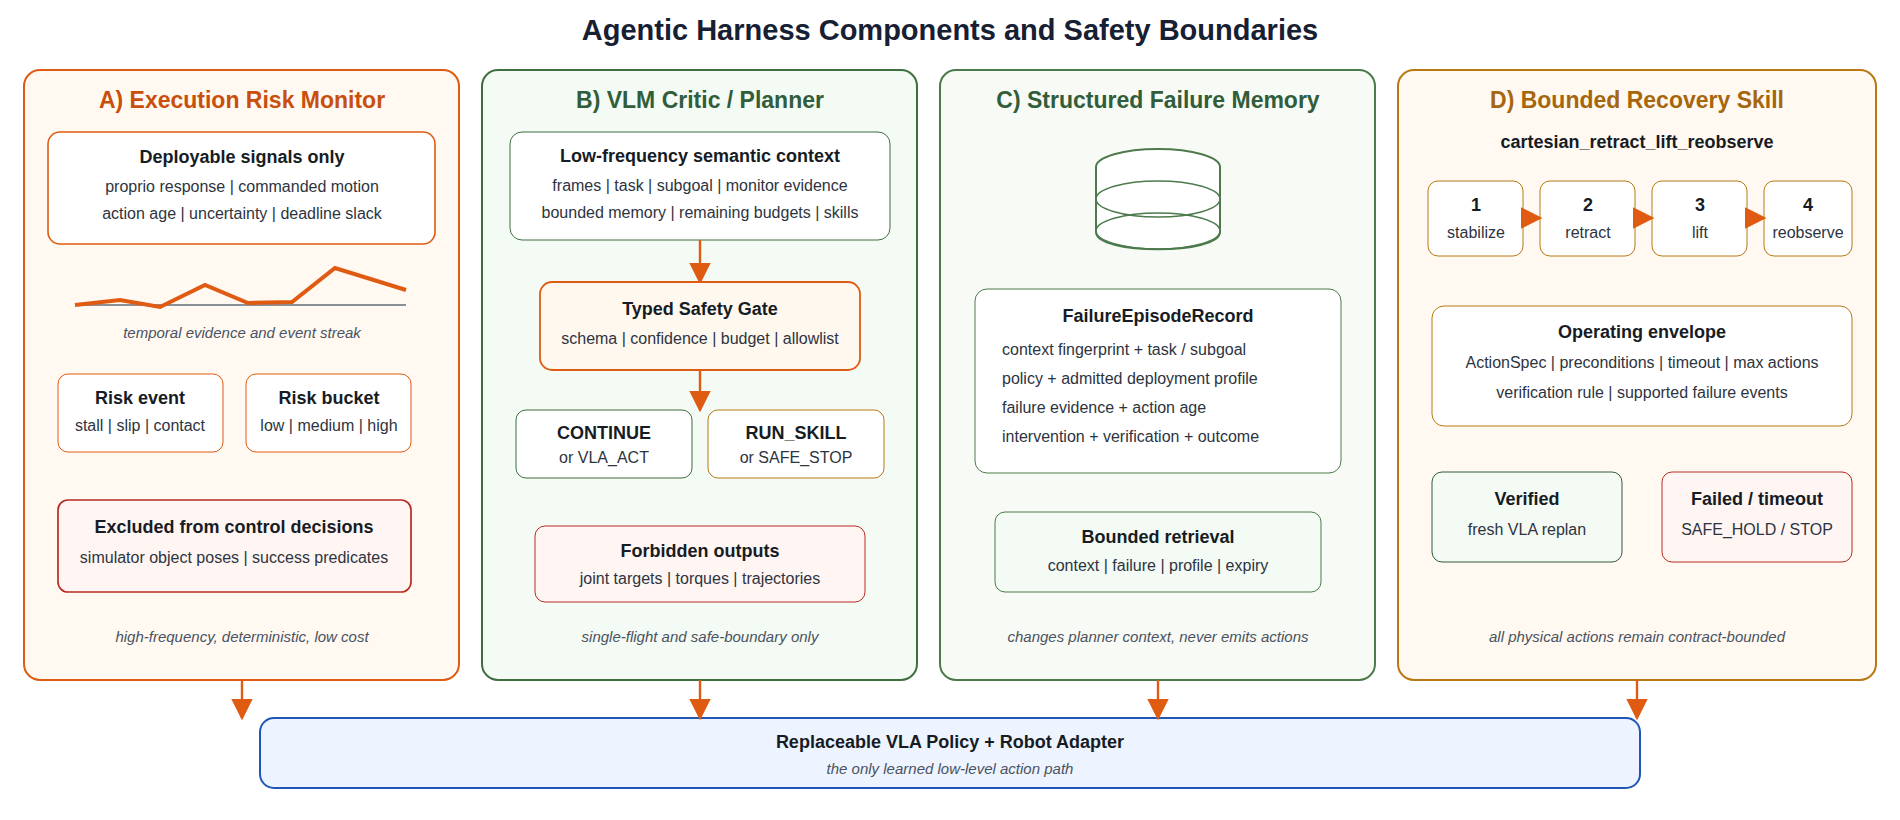
\includegraphics[width=0.94\textwidth]{figures/fig3_modules_v2.png}
    \caption{Agentic Harness components and safety boundaries. The Monitor,
    VLM Planner, structured memory, and physical recovery skill have distinct
    inputs, rates, outputs, and authority. Only the replaceable VLA policy
    produces learned low-level actions.}
    \label{fig:modules}
\end{figure}

\subsection{Evidence-Gated Optimize Runtime}

Long-horizon supervision is useful only if the control loop remains feasible
under robot timing and memory constraints. \method{} separates \emph{offline
profile admission} from \emph{online execution}. A VLA profile binds the
checkpoint, robot adapter, hardware, precision, backend, flow-step count, and
action horizon; a Planner profile binds its VLM, prompt, output schema, and
token budget. Thus, a faster backend cannot silently change the policy,
planner contract, or robot interface.

Candidates pass three gates: (i) VLA action fidelity or Planner schema and
intent validity, (ii) warm latency, deadline, VRAM, and co-resident runtime,
with cold start reported separately, and (iii) paired closed-loop task,
recovery, and safety outcomes. Only a promoted manifest is executable;
rejected profiles remain negative evidence.

Formally, profile $p$ is admitted only when
\begin{equation}
\mathrm{Admit}(p)=G_{\mathrm{contract}}(p)\wedge
G_{\mathrm{fidelity}}(p)\wedge G_{\mathrm{runtime}}(p)\wedge
G_{\mathrm{closed}}(p).
\label{eq:admission}
\end{equation}
The contract gate checks model family, checkpoint digest, hardware identity,
adapter, action semantics, precision, flow-step count, horizon, and view
contract. Fidelity compares first action, complete chunk, cosine similarity,
gripper mode, cumulative endpoint, and action jerk under paired fixed noise.
Runtime reports cold preparation separately from warm P50/P95/P99, deadline
misses, and peak VRAM. The closed-loop gate restores identical simulator states
and requires accepted task, recovery, and safe-stop outcomes. Passing replay
fidelity alone is therefore insufficient.

Online requests receive a typed receipt, capability negotiation, prepared
backend, deadline decision, and narrow fallback. Traces separate \emph{model
latency}, \emph{reaction latency} from event to accepted intervention, and
\emph{task-cycle latency} including sensing, execution, waits, and controller
overhead. The same contract rejects asynchronous prefetch after closed-loop
regression. The admitted default is synchronous compiled BF16 with calibrated
sampling and static masked-view elision when the adapter proves a permanently
padded view.

Static masked-view elision (SMVE) is a contract-specific optimization rather
than generic image dropping. Some \pizero{} observation schemas always contain
a named padded camera slot with an all-false mask. After validating this
identity on every request, SMVE removes the inactive tensor before visual
embedding and prefix construction, then compiles the shortened sampler. If the
view becomes active, only this mask-contract violation falls back to a
separately admitted compiled-BF16 profile; OOM, NaN, and unrelated runtime
errors remain visible. This narrow fallback prevents an optimization from
silently masking a system fault.

The online call path is therefore
\begin{quote}
request $\rightarrow$ capability negotiation $\rightarrow$ admitted profile
$\rightarrow$ action validation $\rightarrow$ deadline receipt $\rightarrow$
trace/fallback record.
\end{quote}
Unsupported controls are either rejected or explicitly recorded as dropped.
For example, \pizero{} supports flow-step control and chunks, whereas OpenVLA
exposes autoregressive single-action decoding and does not pretend to support
the same controls.

\begin{figure}
    \centering
    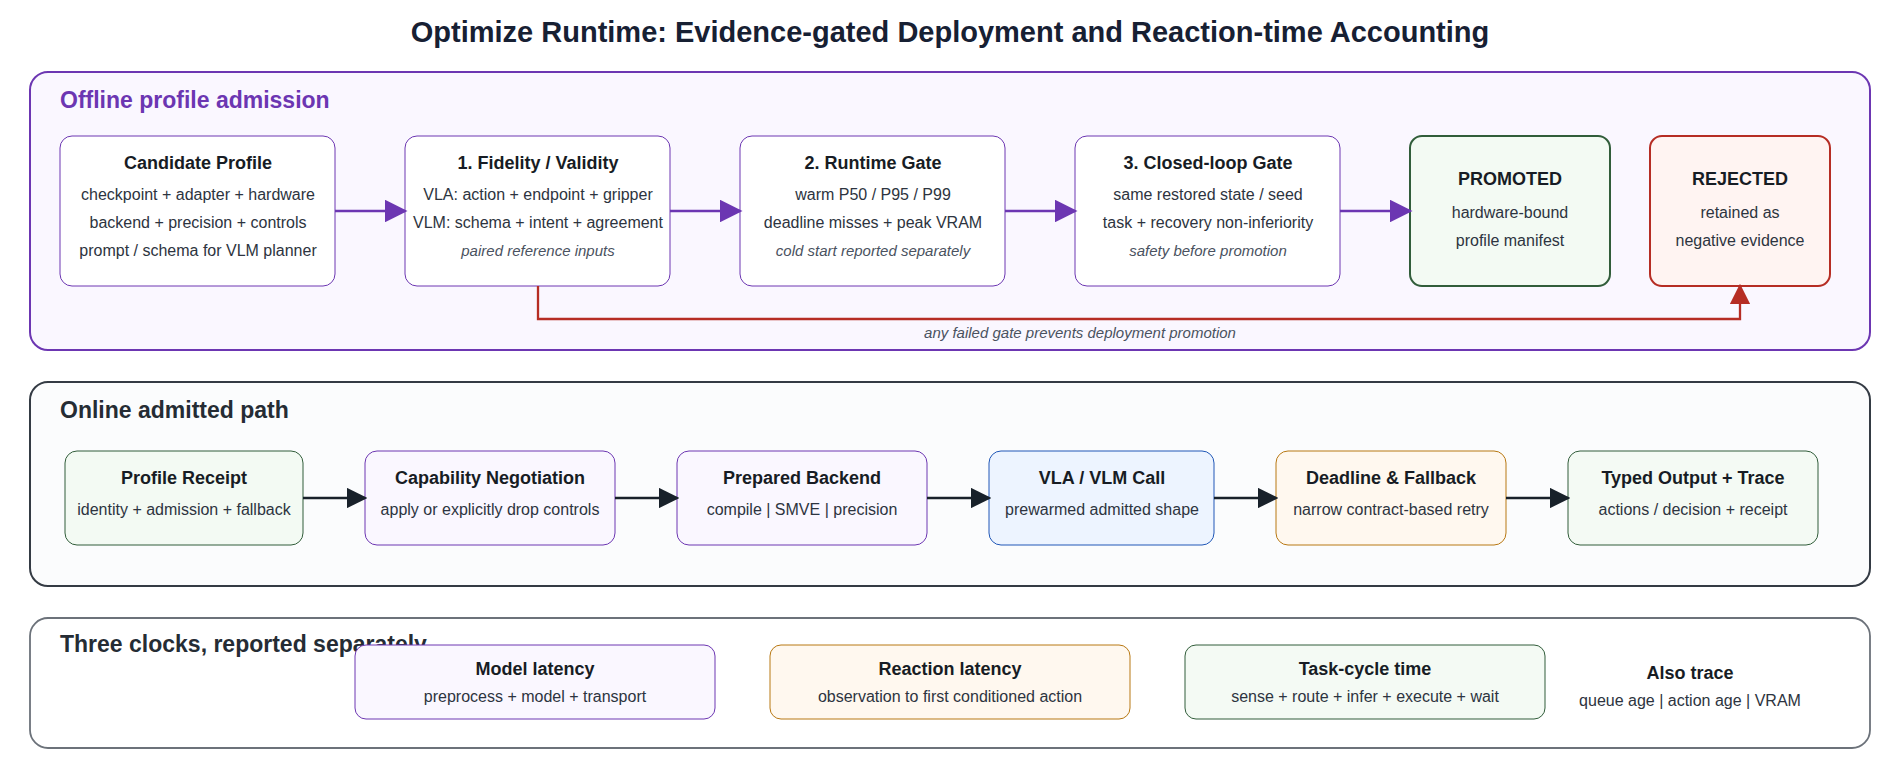
\includegraphics[width=0.94\textwidth]{figures/fig4_realtime_runtime_v2.png}
    \caption{Optimize Runtime separates offline profile admission from online
    execution. A backend is promoted only after fidelity or validity, runtime,
    and closed-loop gates; online traces distinguish model, reaction, and
    task-cycle latency.}
    \label{fig:runtime}
\end{figure}

\subsection{End-to-End Runtime Procedure}

For clarity, one episode executes the following procedure.
\begin{enumerate}
    \item Normalize sensor data through the robot adapter and validate the
    observation/action contract. The evaluator may retain privileged state for
    scoring, but the Harness does not receive it.
    \item Update the high-rate Monitor from commanded action, proprioceptive
    response, optional frame difference, action age, uncertainty, and deadline
    slack.
    \item If risk is low, execute the remaining validated chunk. If a fresh
    call is needed, negotiate controls with the admitted VLA profile, infer one
    chunk, validate it, and attach its runtime receipt.
    \item On a confirmed event, clear stale actions and route by failure streak,
    skill coverage, and remaining budgets. The choices are a fresh VLA replan,
    one bounded skill, or a VLM safe boundary.
    \item At a VLM boundary, retrieve only matching, unexpired memory and HAA
    records, enter safe hold, issue a single-flight multimodal request, and
    apply only an accepted typed intent. Planner cooldown prevents repeated
    calls from turning semantic reasoning into the control loop.
    \item Verify physical response after a skill, write a typed outcome record,
    and either replan from the new observation or fail closed. Every transition
    records model, reaction, task-cycle, queue-age, action-age, budget, and
    fallback evidence.
\end{enumerate}
This procedure also explains why Agentic and efficient inference are coupled:
recovery and replanning add calls exactly when the robot is off nominal, while
semantic planning adds a second model with a seconds-scale boundary latency.
Optimizing only nominal VLA throughput would miss the costly path that matters
most during failure.

\section{Experimental Design}
\label{sec:experiments}

\subsection{Evidence Hierarchy}

We separate five evidence tiers. The benchmark tier is a full paired study over
four official suites. Each method receives the same 10 policy-noise states for
each of 10 tasks in clean \texttt{libero\_10}, Object-OOD, Swap-OOD, and
Task-OOD, yielding 400 episodes per method and 1,200 episodes overall. The
mechanism tier retains earlier LIBERO-10 weak-task, exact-state recovery, and
guarded-VLM tests because they expose why individual outcomes change. The VLA
deployment tier measures five PI0.5 profiles on 45 paired observations. The
Planner deployment tier compares BF16, INT8, and NF4 Qwen3.5-4B profiles on the
same 30 temporal observations. Finally, the coupling tier loads one admitted
Planner and VLA profile concurrently and validates the typed handoff and
resource envelope. Simulator state is used only for evaluator-side restoration
and labels, never by the online controller. This hierarchy prevents an
open-loop match, kernel timing result, or one successful intervention from
being reported as embodied task success.

\begin{table}
\caption{Evaluation design and claim boundary.}
\label{tab:evidence}
\centering
\small
\begin{tabularx}{\textwidth}{p{0.18\textwidth}p{0.38\textwidth}X}
\toprule
Tier & Protocol & Role in paper \\
\midrule
Benchmark & 4 suites $\times$ 10 tasks $\times$ 10 states $\times$ 3 methods & paired success, compute, and intervention evidence \\
Mechanism & historical weak tasks and restored failures & diagnose transitions, recovery, and VLM handoff \\
VLA deployment & 45 observations; 5 PI0.5 profiles & fidelity, latency, VRAM, and 80-ms deadline gate \\
Planner deployment & 30 temporal observations; 3 precisions & protocol validity and semantic-decision agreement \\
Coupling & co-resident NF4 Planner and SMVE VLA & typed handoff and single-GPU feasibility only \\
\bottomrule
\end{tabularx}
\end{table}

\subsection{Metrics and Configurations}

The main metric is task success from the simulator completion signal. Agentic
runs additionally report interventions, recovery phase and outcome, action
count, and episode length. Runtime traces separate model, reaction, and
task-cycle latency, and also retain deadline misses, wall time, peak VRAM, and
safe-boundary waits. Every model call records requested, applied, dropped, and
fallback controls together with deployment-profile identity and the triggering
Agentic event. Each reported runtime uses warmup and fixed noise; videos and
JSONL traces are retained.

The baseline is the unmodified \texttt{pi05\_libero} checkpoint. The full
paired benchmark compares Frozen VLA, Fixed Recovery, and Full Agentic. Full
Agentic contains the high-rate Monitor, one bounded recovery skill, guarded
Qwen3.5-4B calls, typed memory/knowledge, and safe stop. It receives no object
pose, task-completion flag, or simulator failure label. Runtime experiments use
the same PyTorch checkpoint. The admitted fidelity-first profile uses two flow
steps, ten committed actions, compiled BF16, and synchronous control.
When an adapter guarantees a permanently padded camera slot, static masked-view
elision (SMVE) asserts its all-false mask and removes it before visual encoding
and prefix-KV construction.
An asynchronous candidate adds two-action, risk-gated prefetch; its causal
control uses synchronous commit eight because both execute eight newly
predicted actions per aligned chunk. It is not promoted unless the closed-loop
gate passes.

\subsection{Implementation and Reproducibility Settings}

The primary action model is the local PyTorch
\texttt{pi05\_libero} checkpoint served through OpenPI. Unless stated
otherwise, the promoted profile uses BF16, two flow steps, horizon/commitment
ten, synchronous execution, and SMVE with ordinary compiled BF16 as its
mask-contract fallback. The external semantic model is Qwen3.5-4B behind an
OpenAI-compatible multimodal endpoint. BF16 is the latency-default profile;
NF4 is separately admitted as a low-memory candidate. The default planner policy is
\texttt{event\_only}; task-start planning is disabled unless an experiment
explicitly selects \texttt{startup\_shadow} or \texttt{startup\_wait}.

The PRO qualification uses at most one physical recovery and two VLM calls per
episode, a 50-step planner cooldown, a 256-token response budget, a 15-s safe
boundary timeout, and a 60-control-step monitor warm-up. VLM decisions below
0.55 confidence, unknown skills/intents, raw action fields, stale tickets, and
malformed JSON fail closed. Fixed policy noise and seeds are shared by compared
branches. The robot action is normalized 7-D delta Cartesian control; each
bounded recovery executes at most 12 actions in the reported configuration.

Experiments run on one RTX 4090 (24 GB). Replay runtime profiles are measured
without unrelated GPU work unless the experiment explicitly evaluates
co-residency. In co-resident tests, VLA and VLM memory and interference are
reported together. Policy observations remain $256\!\times\!256$; the HD PRO
video uses an independent $720\!\times\!720$ MuJoCo renderer and therefore does
not alter model input. Machine-readable JSON/JSONL stores per-call profile ID,
requested/applied controls, latency, deadline, action age, event, recovery
phases, planner ticket, decision acceptance, and safe-stop/fallback fields.

\section{Results}
\label{sec:results}

\subsection{Full Paired LIBERO-PRO Study}

Table~\ref{tab:libero_pro_full} reports the final benchmark study. Every method
is evaluated from the same 400 initial-state/noise pairs. Full Agentic reaches
\CarveFullAgenticSuccess{} versus \CarveFullFrozenSuccess{} for Frozen VLA and
181/400 for Fixed Recovery. Against Frozen VLA, it converts
\CarveFullConversions{} failures and regresses on \CarveFullRegressions{}
previous success. The exact paired McNemar test gives
$p=\CarveFullMcnemar$; consequently, the observed $+0.75$ percentage-point
change is descriptive and is not claimed as a statistically significant
competence gain.

\begin{table}
\caption{Full paired official LIBERO-PRO study. Each suite contains 10 tasks and 10 shared initial states per task.}
\label{tab:libero_pro_full}
\centering\footnotesize
\begin{tabular}{lcccccc}
\toprule
Method & Clean & Object & Swap & Task & Overall & VLA calls \\
\midrule
Frozen VLA & 96/100 & 66/100 & 11/100 & 7/100 & 180/400 & 16,047 \\
Fixed Recovery & 97/100 & 67/100 & 11/100 & 6/100 & 181/400 & 14,442 \\
Full Agentic & 97/100 & 68/100 & 11/100 & 7/100 & 183/400 & 14,699 \\
\bottomrule
\end{tabular}
\end{table}


The compute and intervention outcomes are nevertheless measurable. Full
Agentic reduces executed steps by \CarveFullStepReduction{} and VLA calls by
\CarveFullCallReduction{} relative to Frozen VLA. It invokes 173 bounded
recoveries, issues 263 guarded Planner calls, and safe-stops 84 unsupported or
budget-exhausted episodes. The action model retains a
\CarveFullVlaPninetyfive{} P95; the event-triggered Planner has an
\CarveFullPlannerPninetyfive{} P95 and therefore remains outside the high-rate
control path. Total episode wall time grows by 16.5\% because semantic
reasoning is expensive. These results distinguish two claims: the Harness
reduces unnecessary VLA execution and safely exercises the complete semantic
path, while the present Planner does not establish a significant aggregate
success improvement.

Suite difficulty also exposes the current boundary. Frozen/Full Agentic obtain
96/97 successes on clean tasks and 66/68 on Object-OOD, but both remain at
11/100 on Swap-OOD and Full Agentic remains at 7/100 on Task-OOD. A process
controller can correct selected execution failures; it cannot manufacture
missing OOD manipulation competence in the frozen policy.

\subsection{Historical LIBERO-10 Diagnosis}

Before the full paired study, a 20-state-per-task LIBERO-10 precursor was used
to locate failure modes and develop the Harness. Table~\ref{tab:main} reports
this diagnostic result rather than the final benchmark claim.
The verified baseline reaches 90.0\% (180/200), indicating that the frozen policy is already strong.
The refined deterministic Harness precursor reaches 92.5\% (185/200).
Its value is mechanistic: the backbone is unchanged and the exposed weak task
motivates transition and recovery tests. It is not combined statistically with
the later 1,200-episode protocol.

\begin{table}
\caption{Historical diagnostic comparison on \texttt{libero\_10}.}
\label{tab:main}
\centering
\small
\begin{tabular}{lcc}
\toprule
Method & Success & Episodes \\
\midrule
\texttt{pi05\_libero} & 90.0\% & 180/200 \\
Deterministic Harness precursor & \textbf{92.5\%} & \textbf{185/200} \\
\bottomrule
\end{tabular}
\end{table}

The per-task pattern in Fig.~\ref{fig:libero_task} and Table~\ref{tab:per_task} is more informative than the aggregate alone.
The dominant weak task improves from 55.0\% to 75.0\%.
Most saturated tasks remain stable, while small task-dependent fluctuations persist.
This supports a restrained interpretation: \method{} is not a uniformly beneficial wrapper, but a process-control layer that is most useful when the baseline has visible long-horizon weakness.

\begin{figure}
    \centering
    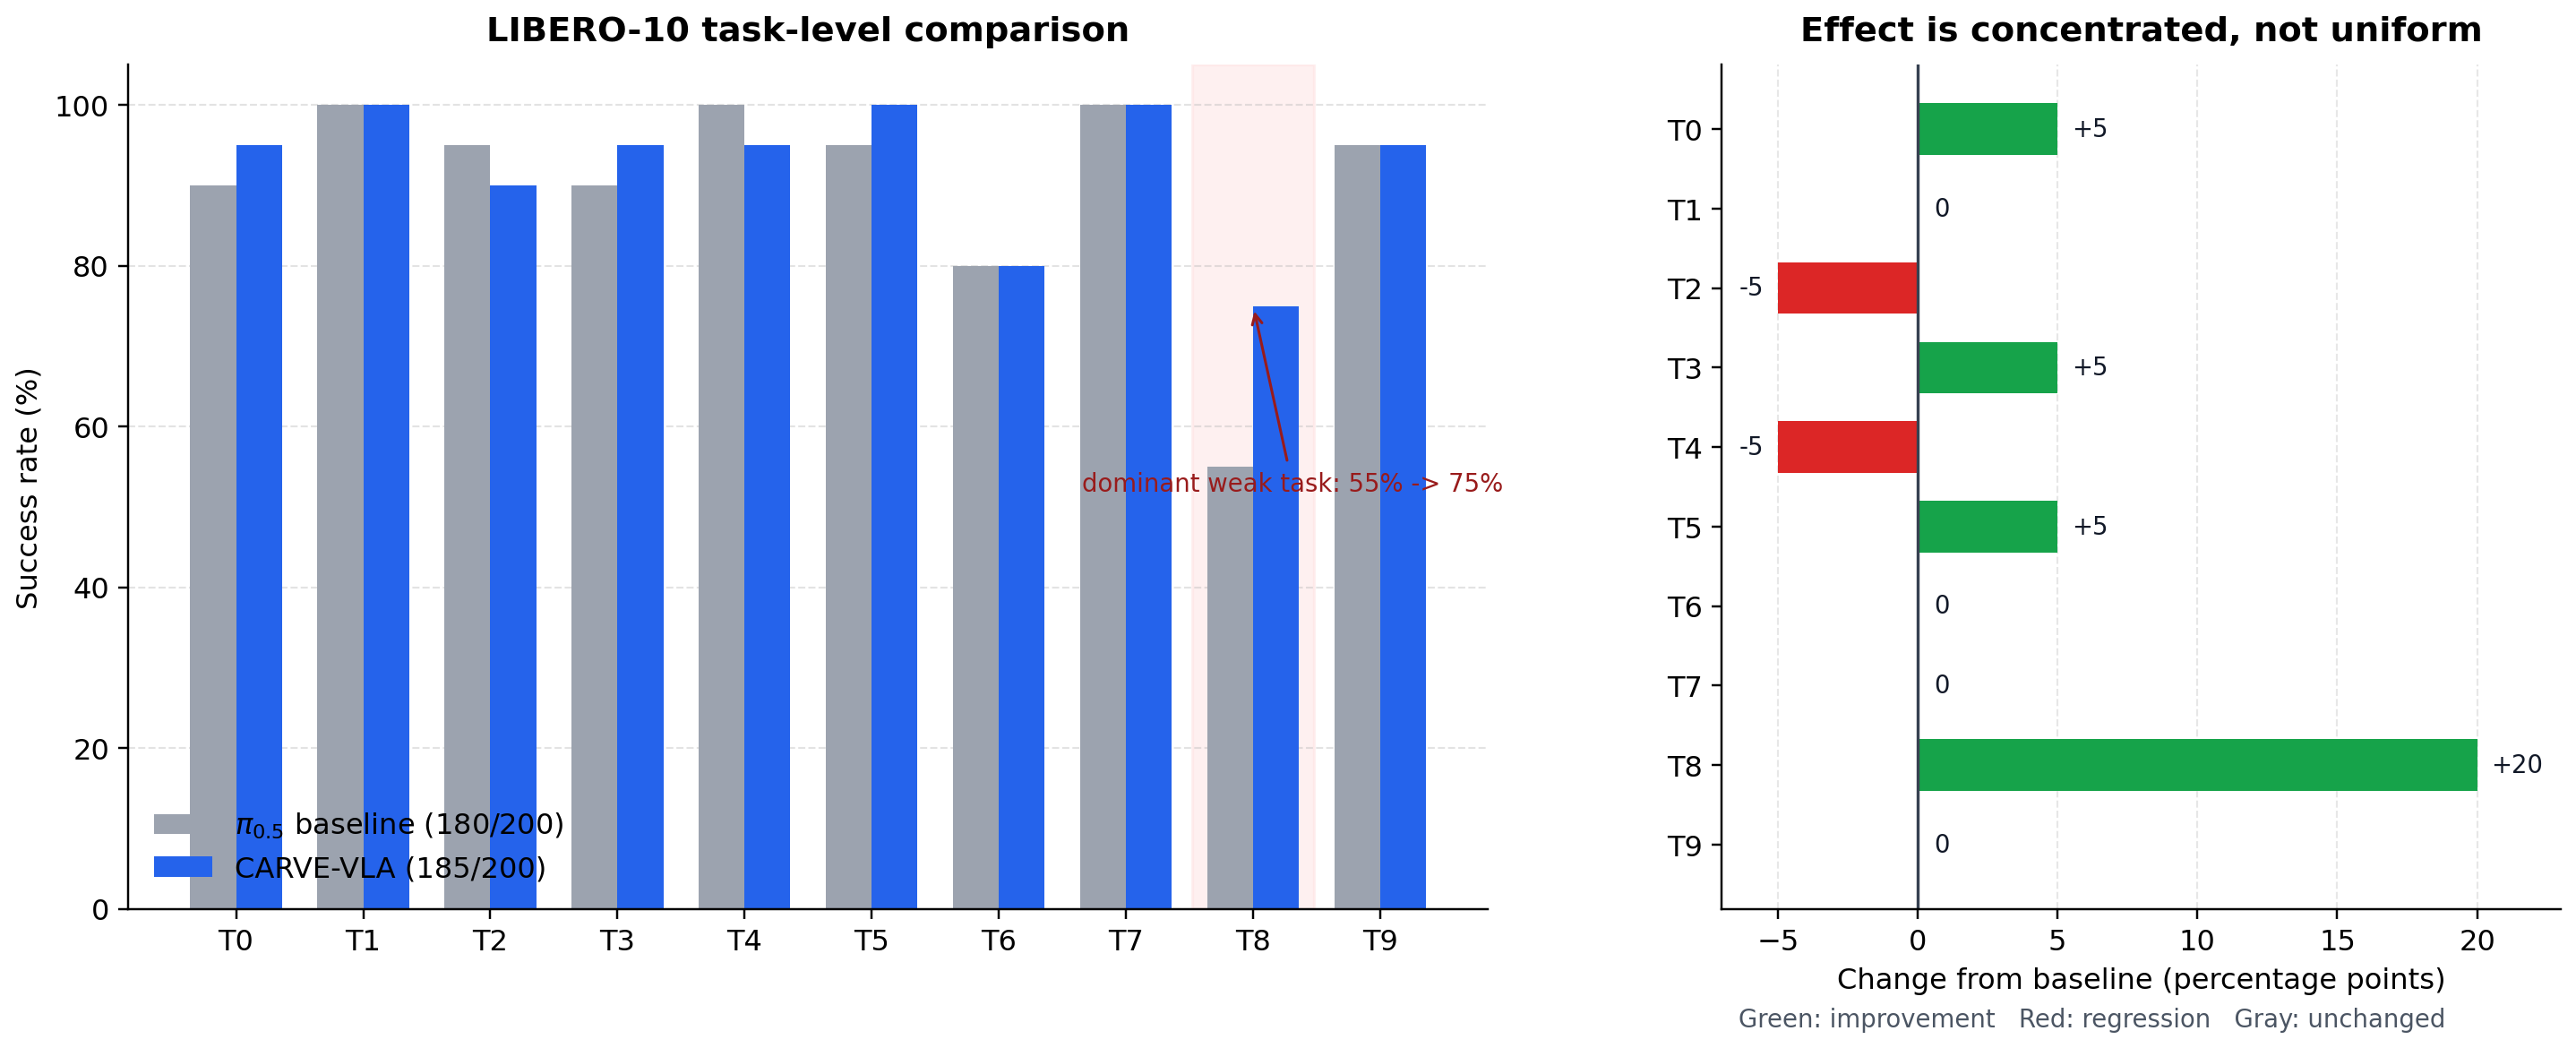
\includegraphics[width=0.94\textwidth]{figures/fig5_libero10_task_comparison_v2.png}
    \caption{Task-level comparison on \texttt{libero\_10}.
    The left panel reports success for 20 episodes per task and method; the
    right panel shows the corresponding change in percentage points. The main
    gain is concentrated in T8 rather than distributed uniformly across
    saturated tasks.}
    \label{fig:libero_task}
\end{figure}

\begin{table}
\caption{Per-task success on \texttt{libero\_10}. Values are percentages.}
\label{tab:per_task}
\centering
\small
\begin{tabular}{lcccccccccc}
\toprule
Method & T0 & T1 & T2 & T3 & T4 & T5 & T6 & T7 & T8 & T9 \\
\midrule
\texttt{pi05\_libero} & 90 & 100 & 95 & 90 & 100 & 95 & 80 & 100 & 55 & 95 \\
Deterministic Harness precursor & \textbf{95} & 100 & 90 & \textbf{95} & 95 & \textbf{100} & 80 & 100 & \textbf{75} & 95 \\
\bottomrule
\end{tabular}
\end{table}

\subsection{Weak-Task Diagnosis and Ablation}

The weak-task subset is the most useful diagnostic regime because saturated tasks hide process-control differences.
Table~\ref{tab:weak} summarizes the targeted follow-up on T6/T8/T9.
After the original full-stack configuration exposed the weak region, a task-targeted v2 follow-up reaches 90.0\% on T6, 70.0\% on T8, and 100.0\% on T9.
This run should be interpreted as targeted repair of exposed failure modes, not as a new suite-level claim.

\begin{table}
\caption{Targeted weak-task diagnosis. Values are percentages.}
\label{tab:weak}
\centering
\small
\begin{tabular}{lccc}
\toprule
Method & T6 & T8 & T9 \\
\midrule
\texttt{pi05\_libero} & 80 & 55 & 95 \\
Original full & 80 & 40 & 90 \\
Task-targeted v2 & 90 & 70 & \textbf{100} \\
Transition only & \textbf{100} & \textbf{80} & 90 \\
Priors/memory only & 80 & 60 & \textbf{100} \\
Critic only & 90 & 70 & 90 \\
\bottomrule
\end{tabular}
\end{table}

The ablations reveal two important points.
First, scene priors and memory contribute positively on difficult cases: removing them drops T8 performance in the targeted setting.
Second, module interaction is non-trivial.
On T8, Transition-only reaches 80.0\%, higher than the task-targeted full setting.
This does not invalidate the framework; it indicates that the remaining bottleneck is coordination among useful modules rather than the absence of process control.

Mechanism traces support the same diagnosis. In the audited full-stack run,
transition interventions average 0.81 per episode and intervened episodes
succeed in 88.9\% of cases. Critic-triggered retries are absent, so the critic
is retained as an audit/escalation interface rather than credited with the
observed benchmark gain.

\subsection{Canonical Guarded-VLM Handoff}

The preceding benchmark evaluates the deterministic precursor. We therefore
test the canonical VLM path separately instead of retroactively attributing the
185/200 result to it. Two supported restored stall states (T6 and T9) are each
evaluated with policy-noise seeds 7, 17, and 42. Every pair begins from the same
MuJoCo state, executes the same verified 12-action physical recovery, and then
compares direct \pizero{} replanning with exactly one guarded Qwen3.5-4B
\texttt{vla\_act} decision followed by \pizero{} replanning.

\begin{table}
\caption{Canonical post-recovery VLM handoff on two restored states and three
fixed-noise seeds. Steps and VLA calls are descriptive means.}
\label{tab:vlm_pair}
\centering
\small
\begin{tabular}{lccc}
\toprule
Continuation & Success & Mean steps & Mean VLA calls \\
\midrule
Physical recovery $\rightarrow$ VLA & 5/6 & 258.7 & 123.7 \\
Physical recovery $\rightarrow$ guarded VLM $\rightarrow$ VLA & \textbf{6/6} & \textbf{250.3} & \textbf{119.2} \\
\bottomrule
\end{tabular}
\end{table}

All six VLM decisions pass the safety gate and none contains a robot action.
The only outcome difference occurs on T9 seed 42, where direct continuation
reaches the 300-step limit and the VLM-guided branch succeeds in 258 steps with
123 VLA calls. Efficiency effects are otherwise mixed across seeds. Each VLM
call adds roughly 5.4--6.1 s at the safe boundary, and the data contain only
two states rather than independent task samples. Table~\ref{tab:vlm_pair}
therefore establishes a real typed handoff and one paired repair, not a global
VLM success-rate or realtime gain.

\subsection{Flow-Step and Backend Calibration}

Table~\ref{tab:calibration} separates policy sampling from action commitment.
Reducing seven flow steps to two while keeping commitment at ten preserves
14/15 paired successes, lowers mean VLA-call latency from 366.9 to 149.0 ms
(2.46$\times$), and reduces episode wall time from 21.27 to 14.40 s (32.3\%).
The seemingly more adaptive 2/4-step controller reaches only 13/15. We
therefore select the simple two-step profile instead of claiming that more
online compute variation is automatically better.

\begin{table}
\caption{Paired flow-step calibration on 15 T6/T8/T9 episodes.}
\label{tab:calibration}
\centering\small
\begin{tabular}{lcccc}
\toprule
Profile & Success & Call (ms) & VLA/ep (s) & Wall/ep (s) \\
\midrule
Reference: 7 steps, commit 10 & 14/15 & 366.9 & 11.15 & 21.27 \\
Calibrated: 2 steps, commit 10 & 14/15 & 149.0 & 4.44 & 14.40 \\
Dynamic: 2/4 steps, commit 10 & 13/15 & 158.9 & 4.98 & 15.91 \\
\bottomrule
\end{tabular}
\end{table}


The final standalone study repeats the deployment gate from a seven-step BF16
reference and reports all candidates in Table~\ref{tab:efficiency_full}.
Two-step sampling alone reduces P95 from 282.43 to 151.35 ms but still misses
the 80-ms deadline on every call. Compilation lowers P95 to 66.06 ms, and SMVE
reaches \CarveFinalSmvePninetyfive{}, an \CarveFinalSmveReduction{} reduction
from V0. Both pass all 45 paired action checks with no 80-ms misses. Late-layer
INT8 saves 10.7\% memory but reaches 994.74-ms P95 on the current
PyTorch-2.12/TorchAO-0.15 stack, so the runtime rejects it. A historical
PyTorch-2.7.1-compatible receipt reached 71.61 ms and retained 2/2 closed-loop
outcomes; the conflicting result is version-gated rather than generalized.

\begin{table}
\caption{Standalone PI0.5 Optimize Runtime ablation on 45 paired observations.}
\label{tab:efficiency_full}
\centering\footnotesize
\begin{tabular}{llcccc}
\toprule
ID & Profile & P95 & Miss@80 ms & VRAM & Fidelity \\
\midrule
V0 & Eager BF16, 7 steps & 282.43 ms & 100\% & 7.12 GiB & reference \\
V1 & Eager BF16, 2 steps & 151.35 ms & 100\% & 7.12 GiB & reference \\
V2 & Compile BF16, 2 steps & 66.06 ms & 0\% & 6.98 GiB & 45/45 \\
V3 & Compile BF16 + SMVE, 2 steps & 54.67 ms & 0\% & 6.98 GiB & 45/45 \\
V4 & Late-language INT8, 2 steps & 994.74 ms & 100\% & 6.36 GiB & 45/45 \\
\bottomrule
\end{tabular}
\end{table}


The same contract is exercised on autoregressive OpenVLA-7B using ten paired
T8/T9 frames. Eager BF16 reaches P50/P95 of 303.48/310.92 ms at 14.42 GB.
INT8/NF4 lower VRAM to 7.76/4.41 GB, but are slower and match only 50\%/10\%
of action vectors, so both are rejected. Decode accounts for 67.2\% of CUDA
time; exact token-mask alignment and prewarmed LLM compilation reduce P50/P95
to 224.25/231.84 ms with 10/10 exact actions. Preparation takes 200.19 s and
all calls still exceed 100 ms, making this a scoped speedup, not a 10-Hz claim.

In the paired synchronous T8/T9 gate, SMVE reaches \CarveSmveSuccess{} versus
\CarveSyncEightSuccess{} and reduces wall time from 205.79 to 199.12 s. This
is treated as behavior-preservation evidence, not a statistically supported
task-competence improvement.

\subsection{Planner Quantization and Low-Memory Coupling}

Planner optimization has a different objective from VLA optimization because
it runs only at safe boundaries: semantic fidelity and memory capacity are
primary, while seconds-scale latency is acceptable but still measured.
Table~\ref{tab:planner_quant} compares three Qwen3.5-4B profiles on the same 30
temporal observations. All produce protocol-valid outputs, zero no-op false
positives, full severe-intervention recall, and 100\% exact semantic-decision
agreement. BF16 is the latency default. NF4 reduces allocated model memory by
\CarvePlannerNfMemoryReduction{} at a 53.4\% P95 latency penalty and is retained
as a low-memory tier. INT8 is rejected because the current batch-one kernel is
3.43$\times$ slower than BF16 despite its lower memory.

\begin{table}
\caption{Qwen3.5-4B Planner precision ablation on 30 paired temporal observations.}
\label{tab:planner_quant}
\centering\small
\begin{tabular}{llcccc}
\toprule
ID & Precision & VRAM & P95 & Agreement & Decision \\
\midrule
Q0 & BF16 & 8.46 GiB & 1.90 s & 100\% & latency default \\
Q1 & INT8 & 4.84 GiB & 6.50 s & 100\% & kernel rejected \\
Q2 & NF4 & 3.08 GiB & 2.91 s & 100\% & memory tier \\
\bottomrule
\end{tabular}
\end{table}


The low-memory integration gate concurrently loads the NF4 Planner and SMVE
PI0.5 services on one RTX 4090. The measured process allocation is
\CarveLowMemoryPair{}. One real image-conditioned Planner request is accepted
as typed \texttt{vla\_act}; PI0.5 then emits a valid $10\!\times\!7$ action
chunk in \CarveLowMemoryVlaLatency{}, below the 80-ms VLA-call deadline, with
no fallback. The primitive boundary deliberately withholds these actions from
the simulator. We therefore classify this as an integration pass with system
admission pending, not as a closed-loop task-success result.

\subsection{Physical Recovery and Closed-Loop Gating}

Replay acceptance is necessary but not sufficient. From the same restored T6
stall state, compiled BF16 accurate replanning fails at the 280-step horizon,
whereas a two-call Agentic retry succeeds in 235 steps and bounded physical
recovery plus replan succeeds in 236. Repeating the physical branch reproduces
success, step count, 112 VLA calls, 12 recovery actions, and final-state digest.
The online sentinel further executes first-stall replanning, repeated-stall
physical recovery, response verification, and post-recovery replanning in one
controller lifecycle; it succeeds with a 0.0180-m end-effector response and
zero policy-call deadline misses.

A broader exact-state challenge restores T6/T9 stalls and one unsupported T8
\texttt{stale\_action} state. Table~\ref{tab:recovery_challenge} shows why
indiscriminate retries are not a useful Agentic mechanism: frequent replanning
and prompt retry use 452 and 508 VLA calls versus 113 for frozen continuation,
yet all three retain the same 2/3 success. Physical recovery executes on the
two covered stalls, verifies both, and deliberately safe-stops before issuing
an action on the unsupported T8 event. Equal success is not presented as an
improvement; reduced unnecessary compute and explicit skill coverage are the
result.

\begin{table}
\caption{Exact-state PI0.5 recovery challenge in LIBERO MuJoCo.}
\label{tab:recovery_challenge}
\centering\small
\begin{tabular}{lcccc}
\toprule
Intervention & Success & VLA calls & Executed & Safe stop \\
\midrule
Frozen continuation & 2/3 & 113 & 3/3 & 0 \\
Frequent replan & 2/3 & 452 & 3/3 & 0 \\
Prompt retry & 2/3 & 508 & 3/3 & 0 \\
Physical recovery & 2/3 & 251 & 2/3 & 1 \\
\bottomrule
\end{tabular}
\end{table}


The W8A16 profile loses the compiled-BF16 T6 recovery success despite passing
all replay checks and satisfying the latency deadline. It is therefore rejected
by the closed-loop gate. This negative result is important for lightweight VLA
deployment: small action error can accumulate into a different intervention
outcome even when open-loop aggregate metrics appear acceptable. Compiled BF16
remains the default. On the corrected synchronous commit-10 held-out T8/T9
gate, the controller completes \CarveSyncTenSuccess{} tasks and verifies
\CarveSyncTenRecovery{} physical recovery attempts.

The direct Agentic--Optimize coupling test then runs the same T6/T9 physical
recovery states under eager BF16, compiled BF16, and compiled BF16 with SMVE.
All profiles retain 2/2 task outcomes and 2/2 verified recoveries, while the
admitted profiles remove every 80-ms model-call miss. This is the cleanest
evidence that inference optimization accelerates the failure path rather than
only nominal standalone calls.

\begin{table}
\caption{Same-state Agentic recovery under PI0.5 runtime profiles.}
\label{tab:agentic_optimize}
\centering\small
\begin{tabular}{lcccc}
\toprule
Profile & Success & Recovery & P95 (ms) & 80-ms miss \\
\midrule
Eager BF16 & 2/2 & 2/2 & 166.26 & 236/236 \\
Compiled BF16 & 2/2 & 2/2 & 65.75 & 0/239 \\
Compiled BF16 + SMVE & 2/2 & 2/2 & 54.50 & 0/247 \\
\bottomrule
\end{tabular}
\end{table}


\subsection{Risk-Gated Asynchronous Execution}

Model-call real time does not imply control-loop real time. In the synchronous
T6 profile, image preparation and MuJoCo stepping raise a 69.09-ms policy P95
to 114.01-ms VLA-step control P95. A repeated single-state pilot verified that
risk-gated prefetch can overlap this critical path; it is implementation
evidence rather than the deployment decision.

The initial two-episode check preserved both successes, but
Table~\ref{tab:prefetch} gives the decisive five-state-per-task expansion.
Full-duty prefetch reduces deadline misses from 417/3931 to 48/4287
(\CarveRealtimeMissReduction{} relative), yet success drops from
\CarveSyncEightSuccess{} to \CarveAsyncSuccess{}. Requiring a fresh synchronous
chunk after every prefetched chunk still reaches only
\CarveAsyncIntervalSuccess{}. The failures are not worker faults: both profiles
have zero inference errors and verified physical recoveries, but temporally
shifted observations alter the subsequent VLA trajectory. We therefore reject
asynchronous prefetch from the promoted runtime. Compiled BF16 remains the
fidelity-first default, and the residual end-to-end synchronization problem is
left explicit rather than hidden behind model-call latency.

\begin{table}
\caption{Expanded T8/T9 asynchronous-execution gate (ten episodes).}
\label{tab:prefetch}
\centering\footnotesize
\begin{tabular}{lccccc}
\toprule
Execution & Success & Calls & Wall (s) & 80-ms miss & Miss rate \\
\midrule
Sync, commit 8 & 7/10 & 417 & 205.79 & 417/3931 & 10.61\% \\
Async, every chunk & 5/10 & 346 & 198.21 & 48/4287 & 1.12\% \\
Async, alternating & 5/10 & 315 & 207.58 & 176/4278 & 4.11\% \\
\bottomrule
\end{tabular}
\end{table}


\subsection{Focused LIBERO-PRO Mechanism Traces}
\label{sec:pro}

Before launching the full paired study, we used a focused capability screen to
verify that the official suite variants, frozen policy, Planner, Monitor, and
recovery skills could execute together. With three fixed-noise trials per
selected task, frozen \pizero{} obtains 7/9 on clean T3/T8/T9, 4/6 on
Object-OOD T3/T9, 2/9 on Task-OOD T3/T8/T9, and 0/9 on Swap-OOD T3/T8/T9.
These small trials are retained because their traces expose specific natural
events; the aggregate claim comes from Table~\ref{tab:libero_pro_full}.

\begin{table}
\caption{Focused frozen-VLA LIBERO-PRO capability screen. Each selected task
uses three fixed-noise trials; this is not the official full protocol.}
\label{tab:pro_screen}
\centering
\small
\begin{tabular}{lccc}
\toprule
Suite & Selected tasks & Success & Diagnostic role \\
\midrule
Clean & T3, T8, T9 & 7/9 & paired reference \\
Object-OOD & T3, T9 & 4/6 & intermediate candidate \\
Task-OOD & T3, T8, T9 & 2/9 & mostly floor \\
Swap-OOD & T3, T8, T9 & 0/9 & floor for current policy \\
\bottomrule
\end{tabular}
\end{table}

On the paired clean subset, Frozen VLA, Fixed Recovery, and Full Agentic reach
7/9, 8/9, and 8/9, respectively. The same T9 trial fails under Frozen VLA and
succeeds under both recovery variants. Full Agentic makes one real
post-recovery VLM call with the accepted subgoal \texttt{insert mug into
microwave}; because Fixed Recovery also succeeds, this validates the complete
semantic loop but not additional semantic success.

The semantic-first follow-up changes the order from physical-recovery-first to
``VLM decision, then registered skill or grounded VLA replan.'' On three clean
T9 trials, Frozen VLA reaches 2/3, Fixed Recovery 3/3 with one physical
recovery, and Semantic-First Agentic 3/3 with one VLM call and no physical
recovery. In the informative trial, the Harness detects a stall at step 94,
retrieves mug/microwave HAA cards, accepts \texttt{vla\_act} with subgoal
\texttt{close microwave door}, preserves the original task instruction, and
completes the episode. The VLM call takes 8.02 s at the safe boundary while
\pizero{} remains at 54.26-ms mean latency. Thus the architecture successfully
separates semantic latency from the fast action path, but low-frequency VLM
latency remains a deployment bottleneck.

\begin{table}
\caption{Semantic-first clean-T9 qualification with the same three fixed-noise
trials. Calls and recoveries are totals.}
\label{tab:pro_semantic}
\centering
\small
\begin{tabular}{lccc}
\toprule
Method & Success & VLM calls & Physical recoveries \\
\midrule
Frozen VLA & 2/3 & 0 & 0 \\
Fixed Recovery & 3/3 & 0 & 1 \\
Semantic-First Agentic & 3/3 & 1 & 0 \\
\bottomrule
\end{tabular}
\end{table}

Figure~\ref{fig:pro_demo} shows the independent HD demonstration on official
Object-OOD T8, where both standard moka pots are replaced by
yellow assets. All three fixed-seed trials succeed. Trial 0 naturally detects a
stall at step 337, executes and verifies the 12-action preserve-grasp recovery,
replans with the promoted \pizero{} profile, and completes both placements.
Across the three trials, mean/P95 VLA latency is 54.54/58.07 ms. No VLM is
called in this particular demonstration; it isolates Monitor, bounded recovery,
and optimized VLA execution under an observable object shift.

\begin{figure}
    \centering
    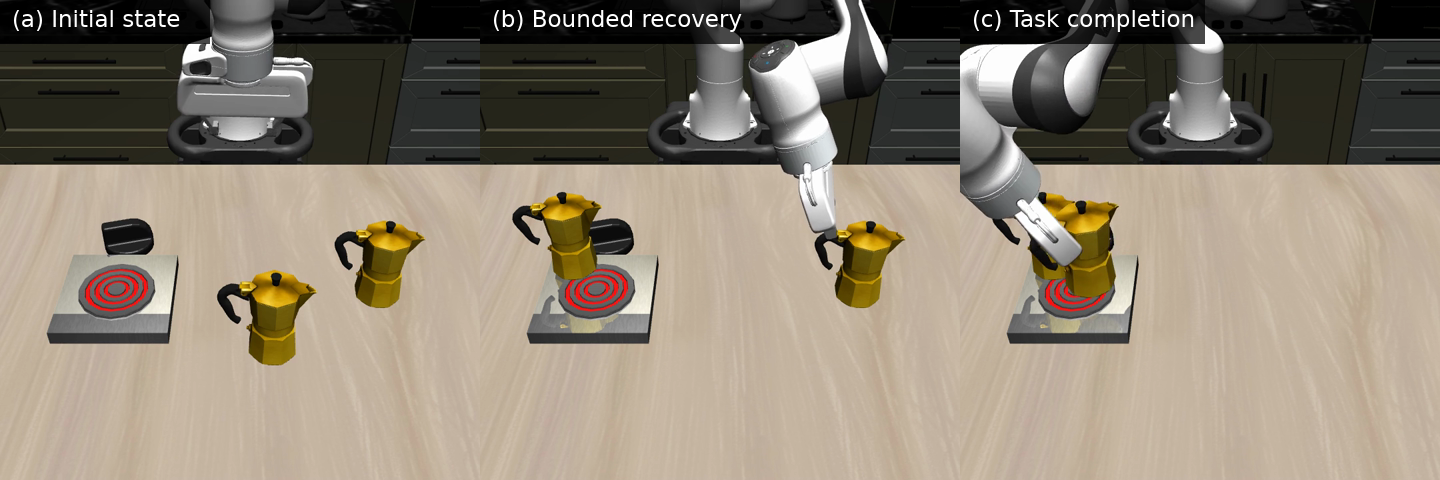
\includegraphics[width=0.98\textwidth]{figures/fig6_libero_pro_t8_recovery.png}
    \caption{Native $720\!\times\!720$ display frames from the successful
    LIBERO-PRO Object-OOD T8 rollout. The model still receives the unchanged
    $256\!\times\!256$ policy observation. The middle frame is sampled during
    the verified bounded recovery; both yellow moka pots satisfy the stove goal
    at termination.}
    \label{fig:pro_demo}
\end{figure}

\section{Discussion and Limitations}
\label{sec:discussion}

\paragraph{Supported claim.}
The full paired study supports a conservative systems claim. A strong frozen
VLA can be wrapped by an external process-control layer that executes guarded
semantic decisions, bounded recovery, memory, and safe stop while reducing
VLA calls by \CarveFullCallReduction{}. The $+3/400$ success difference is not
statistically significant and is not the basis of the contribution. Exact-state
and focused traces instead show where selected failures are corrected and where
the frozen policy remains outside the Harness's skill coverage.
The runtime studies support a complementary deployment claim: lower-step
sampling, compilation, and contract-checked padding elimination preserve paired
actions and closed-loop evidence while bringing PI0.5 calls below 80 ms.
Planner NF4 establishes a practical memory tier, and the co-resident gate shows
that it can share one 24-GB GPU with the admitted VLA profile. Rejected INT8 and
asynchronous profiles show why memory, kernel latency, replay fidelity, and
embodied behavior must be admitted separately.

\paragraph{What is not claimed.}
\method{} is not a new VLA backbone and does not claim universal benchmark dominance.
The current runtime uses explicit risk- and deadline-conditioned scheduling; it
does not claim a learned globally optimal compute-allocation policy or hard
real-time guarantees. SMVE applies only when an adapter guarantees a static
padding view. The OpenVLA result validates the shared adapter, profiling, and
fidelity boundary, not transfer of this PI0.5-specific transform or a universal
speedup.
INT8 and NF4 are standard deployment transforms evaluated inside our gate, not
new quantization algorithms. NF4 supports a positive Planner-memory claim, but
the present PI0.5 INT8 kernel is rejected and does not support a compressed-VLA
claim. Likewise, physical recovery is supplied by the external execution loop
rather than learned by the VLA.
This distinction is central to the paper: the contribution is deciding how a frozen policy should be supervised during execution.

\paragraph{Ablation lesson.}
Useful modules are not automatically additive; routing among memory, recovery,
retry, and plain VLA execution remains open. The current fixed router is
auditable but not learned. A future router should be trained only after each
candidate action has independent admission and sufficiently diverse failure
data; otherwise an MoE-like gate would add complexity without a trustworthy
supervision target.

\paragraph{Scope.}
Benchmark-wide evidence covers the four evaluated official LIBERO and
LIBERO-PRO suites with 10 paired states per task; it is not a claim of transfer
to arbitrary robots or tasks. Calibration, restored-state recovery, canonical
VLM handoff, prefetch, and OpenVLA remain mechanism or deployment evidence.
The low-memory pair has not yet executed actions in closed loop, and the system
has no real-robot experiment. The lightweight PI0.5 result is reduced sampling
compute and visual-prefix work rather than a smaller checkpoint. Broader policy
transfer, repeated co-resident stress testing, action-aware VLA quantization,
and physical deployment remain future work.

\section{Conclusion}
\label{sec:conclusion}

We presented \method{}, a modular runtime that treats frozen-VLA deployment as
a joint process-control and inference-efficiency problem. Across 1,200 paired
interactive episodes, the full Harness safely exercises monitoring, semantic
planning, bounded recovery, memory, and safe stop while reducing VLA calls;
its small aggregate success difference is explicitly non-significant. The
Optimize Runtime promotes two-step compiled BF16 with SMVE at
\CarveFinalSmvePninetyfive{} P95, retains NF4 Qwen3.5-4B as a
\CarvePlannerNfMemoryReduction{} lower-memory Planner tier, and rejects
backend-dependent INT8 and asynchronous profiles that violate latency or
closed-loop gates. A co-resident single-GPU dry run closes the typed
Planner-to-VLA inference path within \CarveLowMemoryPair{}, while remaining
honestly short of task-level admission. Agentic reliability and efficient
inference should be designed, measured, and admitted as one embodied runtime.

\appendix

\section{Interface and Trace Reference}
\label{app:interfaces}

Table~\ref{tab:interfaces} maps paper concepts to the concrete typed records
used by the implementation. These records are model independent: a new policy
family may replace \pizero{} only by implementing the same adapter boundary and
declaring unsupported capabilities honestly.

\begin{table}
\caption{Core runtime records and their purpose.}
\label{tab:interfaces}
\centering
\small
\begin{tabularx}{\textwidth}{p{0.25\textwidth}X}
\toprule
Record & Required semantics \\
\midrule
\texttt{ActionSpec} & dimension, representation, coordinate frame, gripper convention, control frequency, normalization identity, and optional bounds \\
\texttt{ModelCapabilities} & chunking, configurable flow steps, autoregressive decode, KV cache, uncertainty, async support, precision, and maximum horizon \\
\texttt{InferenceRequest} & normalized observation, original instruction, episode/timestep, Agentic event, requested controls, and request ID \\
\texttt{ActionChunk} & validated actions, untouched backend payload, model latency, and optional uncertainty/predictive context \\
\texttt{RuntimeTrace} & requested/applied/dropped controls, profile and fallback receipts, queue/action age, stage/model/reaction/task-cycle latency, deadline, and action count \\
High-level decision & one of four intents, rationale, confidence, optional subgoal/VLA instruction or registered skill, and qualitative scene update \\
Failure record & context/profile identity, failure evidence, attempted intervention, consumed budget, verification, outcome, confidence, timestamp, and expiry \\
\texttt{RecoveryOutcome} & skill/session identity, trigger, attempt, terminal status, actions executed, replan permission, and deployable verification evidence \\
\bottomrule
\end{tabularx}
\end{table}

CARVE reports three clocks rather than labeling all delay as ``inference.'' If
$t_o$ is observation availability, $t_m^0/t_m^1$ bracket model execution,
$t_a$ is the first action conditioned on that observation, and $t_c$ is cycle
completion, then
\begin{equation}
L_{\mathrm{model}}=t_m^1-t_m^0,\qquad
L_{\mathrm{reaction}}=t_a-t_o,\qquad
L_{\mathrm{cycle}}=t_c-t_o.
\end{equation}
Planner safe-boundary wait belongs to the Agentic/task-cycle trace, not VLA
model latency. Cold model load and compile preparation are also reported
separately from warm steady-state calls.

\section{Key Hyperparameters and Safety Budgets}
\label{app:settings}

\begin{table}
\caption{Primary settings used by the final PI0.5/PRO configuration.}
\label{tab:settings}
\centering
\small
\begin{tabularx}{\textwidth}{p{0.30\textwidth}p{0.20\textwidth}X}
\toprule
Setting & Value & Rationale \\
\midrule
VLA precision/backend & BF16 + compile + SMVE & promoted padded-view profile \\
Flow steps / committed actions & 2 / 10 & paired calibration preserves 14/15 outcomes \\
Policy-call deadline & 80 ms & experimental deployment target, not hard realtime guarantee \\
Monitor window / PRO warm-up & 4 / 60 steps & temporal response with startup-event suppression \\
Risk bucket thresholds & 0.35 / 0.65 & low, medium, and high routing buckets \\
Recovery budget & 1 per episode & prevents repeated analytic interventions \\
Recovery action budget & 12 & 2 stabilize, 4 retract, 4 lift, 2 reobserve \\
Planner policy / cooldown & event-only / 50 steps & keep VLM outside routine control \\
Planner call / token budget & 2 / 256 & bound semantic compute and context growth \\
Boundary timeout & 15 s & terminate rather than wait indefinitely \\
Minimum intervention confidence & 0.55 & reject uncertain \texttt{vla\_act}/\texttt{run\_skill} \\
\bottomrule
\end{tabularx}
\end{table}

\section{Artifact Map and Reproduction Path}
\label{app:artifacts}

The implementation links each paper claim to a machine-readable artifact,
rather than only a plotted number.
{\footnotesize
\begin{itemize}
    \item Agentic contracts and state machine:\\
    \url{agentic_vla/runtime/}.
    \item Optimization profiles and gates:\\
    \url{agentic_vla/optimization/}\\
    \url{results/carve_efficiency_full_20260826/}.
    \item Full paired study, audit, and per-call traces:\\
    \url{results/libero_pro_full_study_20260825/}\\
    \url{scripts/run_libero_pro_full_study.sh}.
    \item Exact-state recovery:\\
    \url{scripts/run_carve_pi05_recovery_challenge.sh}.
    \item Coupled Agentic--Optimize experiment:\\
    \url{scripts/run_carve_pi05_agentic_optimize_pair.sh}.
    \item Canonical VLM evidence:\\
    \url{results/carve_vlm_recovery_pair_20260727/}.
    \item Planner precision and low-memory coupling:\\
    \url{results/carve_efficiency_full_20260826/planner/}\\
    \url{results/carve_efficiency_full_20260826/coupling/}.
    \item Historical LIBERO-PRO capability screen:\\
    \url{results/libero_pro_capability_screen_seed7/}.
    \item HD Object-OOD results and runner:\\
    \url{results/libero_pro_hd_demo_t8_seed7/}\\
    \url{scripts/run_libero_pro_hd_demo.sh}.
\end{itemize}
}
The full-study runner starts the admitted \pizero{} and Planner services,
executes all method/suite/task/state cells, and writes MP4/JSON/JSONL before
aggregation and audit. Re-running it requires the official LIBERO-PRO checkout,
local \texttt{pi05\_libero\_pytorch} checkpoint, and Qwen3.5-4B weights; it
does not modify the global LIBERO configuration. Paper tables and macros are
regenerated by \url{scripts/build_carve_paper_results.py}.

\section{Evidence-to-Claim Matrix}

\begin{table}
\caption{Interpretation boundaries for the current technical report.}
\label{tab:claims}
\centering
\small
\begin{tabularx}{\textwidth}{p{0.43\textwidth}X}
\toprule
Supported & Not supported \\
\midrule
Full Agentic executes 400 paired episodes, reduces VLA calls by \CarveFullCallReduction{}, and records \CarveFullConversions{} conversions/\CarveFullRegressions{} regression & statistically significant aggregate success improvement ($p=\CarveFullMcnemar$) \\
Compiled BF16 and SMVE preserve 45/45 paired actions and reduce PI0.5 P95 to \CarveFinalSmvePninetyfive{} & hard realtime control or a universal VLA acceleration \\
One guarded VLM handoff repairs a paired T9 seed and all six typed calls execute safely & statistically significant VLM success gain across task distributions \\
Bounded recovery verifies response and fails closed outside skill coverage & a general learned physical-skill library \\
Planner NF4 reduces memory by \CarvePlannerNfMemoryReduction{} with exact decisions & a new quantization algorithm or an admitted INT8 PI0.5 checkpoint \\
NF4 Planner and SMVE PI0.5 share one GPU and complete one typed dry run & closed-loop task success for the low-memory pair \\
Official clean/object/task/swap variants are evaluated over 1,200 total episodes & real-robot or sim-to-real validation \\
\bottomrule
\end{tabularx}
\end{table}

\begin{credits}
\subsubsection{\ackname}
Omitted for double-blind review.

\subsubsection{\discintname}
The authors have no competing interests to declare that are relevant to the content of this article.
\end{credits}

\bibliographystyle{waica}
\bibliography{references}

\end{document}
